\subsection{Class diagram}
	The following graphic is the class diagram that we will use for the specification and the implementation.

	%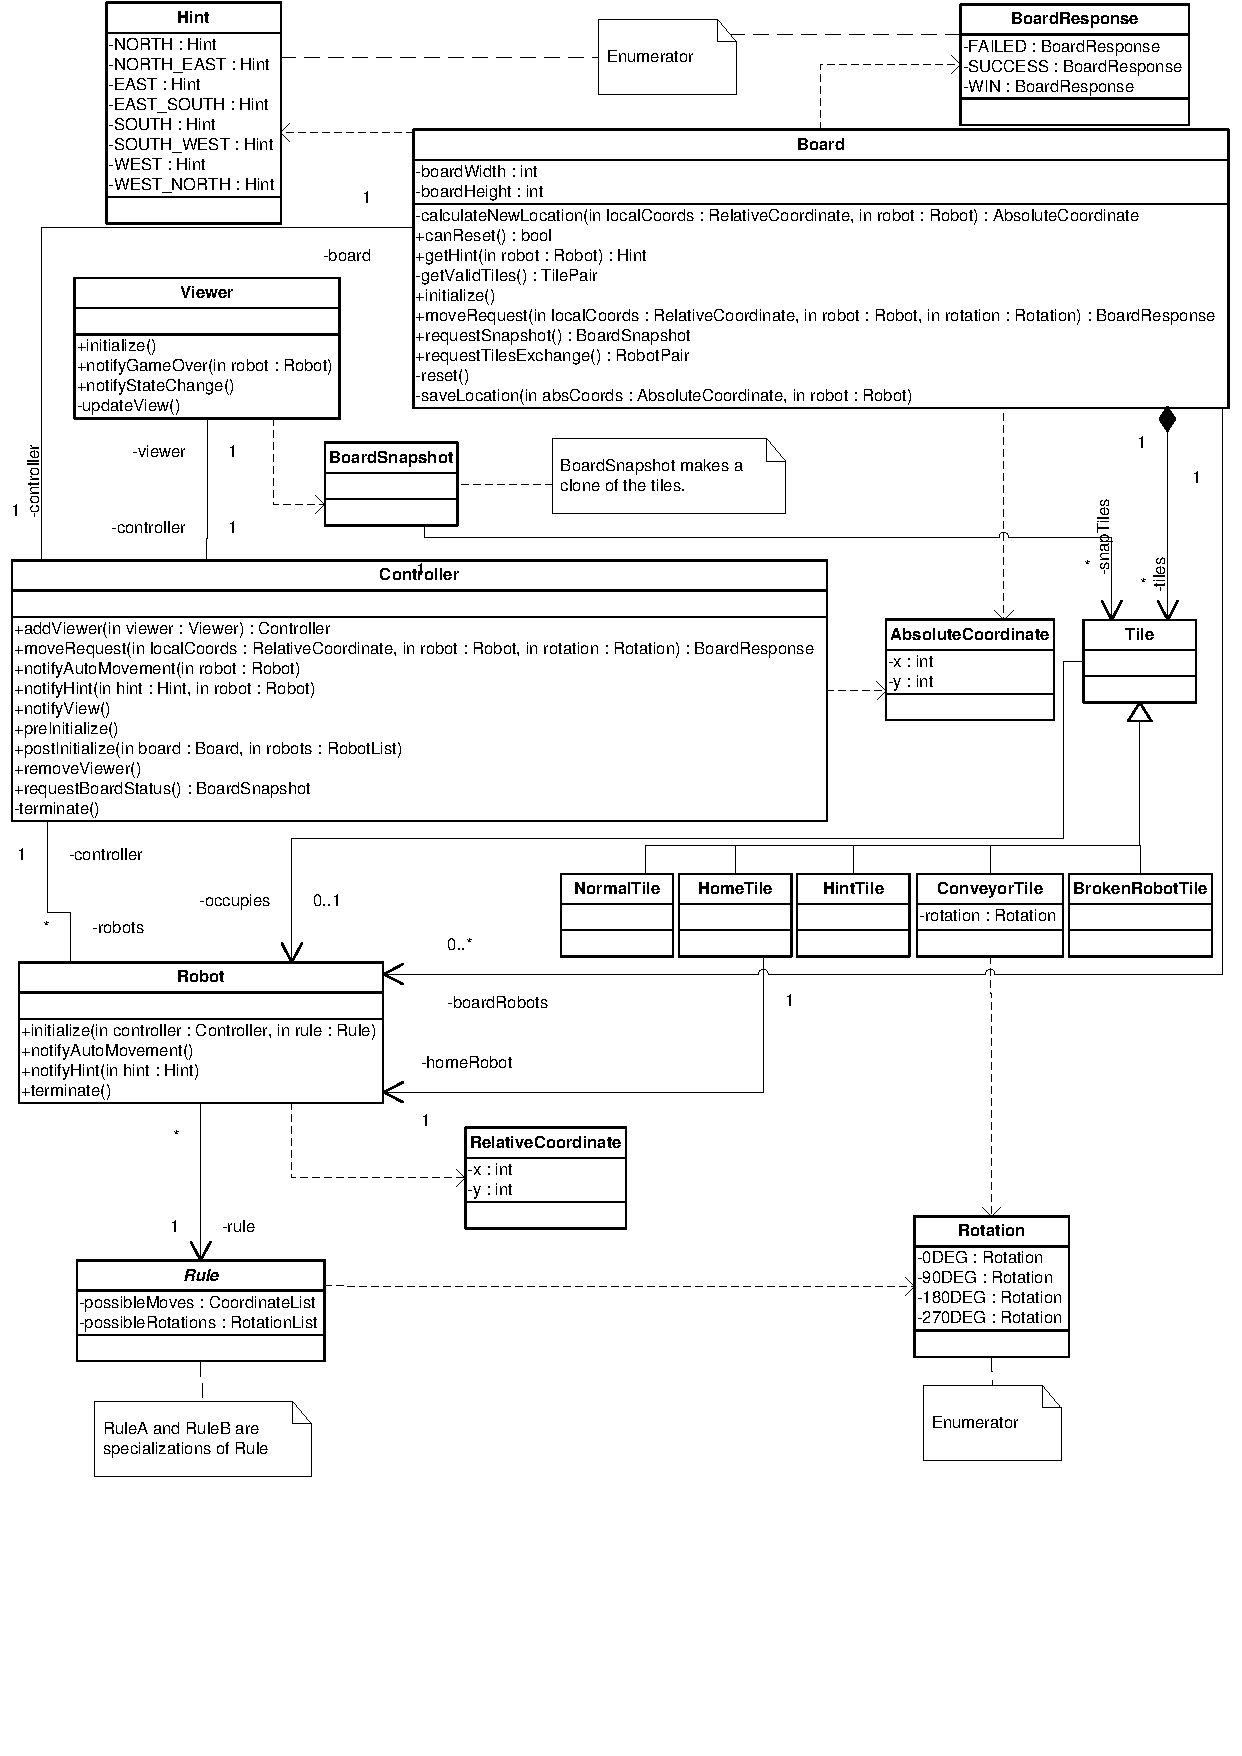
\includegraphics[width=\linewidth]{classdiagram.pdf}
	\let\l=\relax
\let\<=\relax
\let\>=\relax
\digraph[scale=.5]{classdiagram}{
margin=0
fontsize=8
fontname=Helvetica
compound=true
splines=ortho
node [fontsize=8, fontname=Helvetica, shape=record]
edge [fontsize=8, fontname=Helvetica, arrowhead=open, labeldistance=2]
Board [label="{Board|- width : int\l- height : int\l|+ canReset() : bool\l+ initialize()\l+ moveRequest(loc : RelativeCoord, r : Robot, rot : Rotation) : BoardResponse\l+ requestSnapshot() : BoardSnapshot\l+ requestTilesExchange() : bool\l- getHint(r : Robot) : Hint\l- calculateNewLocation(loc : RelativeCoord, r : Robot) :
AbsoluteCoord\l- getValidTiles() : TilePair\l- reset()\l- saveLocation(loc : AbsoluteCoord, r : Robot)\l}"]
Hint [label="{[Hint]| NORTH\l NORTH_EAST\l EAST\l SOUTH_EAST\l SOUTH\l SOUTH_WEST\l WEST\l NORTH_WEST\l}"]
BoardResponse [label="{[BoardResponse]| FAILED\l SUCCESS\l WIN\l}"]
Viewer [label="{Viewer||+ initialize()\l+ notifyGameOver(r : Robot)\l+ notifyStateChange()\l- updateView()\l}"]
BoardSnapshot [label="{BoardSnapshot||}"]
Controller [label="{Controller||+ addViewer(v : Viewer) : Controller\l+ moveRequest(loc : RelativeCoord, r : Robot, rot : Rotation) : BoardResponse\l+ notifyAutoMovement(r : Robot)\l+ notifyHint(h : Hint, r : Robot)\l+ notifyView()\l+ preInitialize()\l+ postInitialize(b : Board, rs : RobotList)\l+ removeViewer()\l+ requestBoardSnapshot() : BoardSnapshot\l- terminate()\l}"]
AbsoluteCoord [label="{AbsoluteCoord|+ x : int\l+ y : int\l|}"]
Tile [label="{Tile||}"]
/**/
subgraph cluster_Tiles {
NormalTile [label="{NormalTile||}"]
HomeTile [label="{HomeTile||}"]
HintTile [label="{HintTile||}"]
ConveyorTile [label="{ConveyorTile|- rot : Rotation|}"]
BrokenRobotTile [label="{BrokenRobotTile||}"]
}
/**/
Robot [label="{Robot||+ initialize(c : Controller, r : Rule)\l+ notifyAutoMovement()\l+ notifyHint(h : Hint)\l+ terminate()\l}"]
RelativeCoord [label="{RelativeCoord|+ x : int\l+ y : int\l|}"]
Rule [label="{\<\<Rule\>\>|- possibleMoves : RelativeCoordList\l- possibleRotations : RotataionList\l|}"]
Rotation [label="{[Rotation]| 0DEG\l 90DEG\l 180DEG\l 270DEG\l}"]
/**/
Board->Controller [taillabel=1, headlabel="0..*"]
Board->Tile [arrowtail=diamond,dir=both, taillabel=1,headlabel="*"]
Board->Robot [taillabel=1, headlabel="0..*"]
/**/
Controller->Viewer [taillabel=1, headlabel=1, arrowhead=none]
Controller->Robot [taillabel=1, headlabel="*", arrowhead=none]
/**/
Tile->Robot [taillabel=1, headlabel="              0..1 - occupier"]
/**/
HomeTile->Robot [taillabel=1, headlabel="              1 - homeRobot"]
/**/
Robot->Rule [taillabel="*", headlabel=1]
/**/
BoardSnapshot->Tile [taillabel=1, headlabel="*"]
/**/
NormalTile->Tile [ltail=cluster_Tiles,arrowhead=empty]
/**/
Board->Hint [style=dashed]
Board->BoardResponse [style=dashed]
Board->AbsoluteCoord [style=dashed]
Viewer->BoardSnapshot [style=dashed]
Controller->AbsoluteCoord [style=dashed]
Robot->RelativeCoord [style=dashed]
Rule->Rotation [style=dashed]
ConveyorTile->Rotation [style=dashed]
} 
    Abstract classes are indicated by guillemets and enumerators by brackets.

\subsection{Class description}
    Next, a description will be given about all the classes in the class diagram. Here, the function of the class can be found, along with its attributes and its functions (and description of these). Since some of the functions have a lot of arguments, these arguments are not showed here. Note that most relations in the class diagram are undirected; for example, the robot has no knowledge about the board, so the association between Board and Robot is directed. The controller and the viewer, however, do have knowledge about each other, so this is an undirected association.

	\begin{description}
        \item[Hint] An enumeration that contains all possible hints that a Robot can receive from a hint tile.
        \item[BoardResponse] An enumerator that contains all the possible responses that the board can give the controller when it makes a move request.
		\item[Board] This class contains the functionality of the board. It contains the following attributes:
        \begin{description}
            \item width: The private variable which contains the width of the board.
            \item height: The private variable which contains the height of the board.
        \end{description}
        Furthermore, we have the following functions:
        \begin{description}
            \item canReset(): The public method which checks if the board can reset. The board can reset if a robot has reached its home tile and a new game can begin.
            \item initialize(): The public method to initialize the board (and with this, also the controller and the robots).
            \item moveRequest(): The public method which handles move requests forwarded by the controller. This method first checks if the move is valid (otherwise, return the BoardResponse FAILED), next it calls calculateNewLocation() to calculate the new location of the robot. After that, saveLocation is called to save the location and the proper board response is returned. Sometimes the board also sends a hint or a notification of an automovement.
            \item requestTilesExchange(): This public method handles with the tiles exchange after a robot has made his move. First it calls getValidTiles() to make sure that the invariant still holds after the exchange. Next it swaps the tiles and handles possible robot replacements or movements.
            \item getHint(): This private method gets an appropriate hint for the robot.
            \item calculateNewLocation(): This private method (used in moveRequest()) calculates the new location of a robot, according to his current position and the position he wants to move to. It also deals with conveyor tiles and broken robot tiles.
            \item getValidTiles(): This private method is used to get two tiles that can be switched, hereby not violating the invariant.
            \item reset(): This private method is used to reset the board. canReset() should return true in order for this function to be called. The board then makes the other components terminate and can initiate new components (e.g. controller, robots) in order to start a new game.
            \item saveLocation(): This private method is used to save the new location of a robot; it is called in moveRequest().
        \end{description}
		\item[Controller] This class represents the controller, which is used as mostly used as communication device between the board and other components. The controller has a viewer, as shown on the undirected association between Controller and Viewer. The controller has the following functions:
        \begin{description}
            \item addViewer(): This public method is used to add a viewer to the controller, so that the controller can notify this viewer when there is a change in the board (see the association in the class diagram).
            \item moveRequest(): This public method is used to forward move requests from the robot. The robot calls this function and the controller calls the moveRequest() function from the board with the right parameters.
            \item notifyAutoMovement(): This public method is used to notify the robot that is has been moved without the robot wanting to; for example, because of a conveyor tile or a tiles exchange.
            \item notifyHint(): This public method is used to notify a robot that it is on a hint tile and what direction he has to go in order to find his home tile.
            \item notifyViewer(): This public method is used to notify the viewer that the board has changed. A snapshot will be send to the viewer.
            \item preInitialize(): This public method is used to pre-initialize the controller, so that there exists an object of the type controller.
            \item postInitialize(): This public method is used to (after pre-initialization) fully initialize the controller with a board and the robots.
            \item removeViewer(): This public method is used to remove a viewer from the controller. This function can be used to add a new viewer or before termination.
            \item terminate(): This function is used to first terminate all objects (except for board). After these objects have been terminated, it informs the board about this; afterwards, the controller itself terminates.
        \end{description}
        \item[Viewer] This class describes the functionality of the viewer, so that the game can be watched. This class has no special attributes. It contains the following functions:
        \begin{description}
            \item initialize(): This public method is used to initialize a viewer.
            \item notifyGameOver(): This public method is used to notify the viewer that a robot has reached its home tile. Fireworks will be shown and after this the viewer can terminate.
            \item notifyStateChange(): This public method is used to notify the viewer that the board has changed, hereby receiving a new snapshot of the board. After this, updateView() will be called to deal with the new snapshot.
            \item updateView(): This private method deals with new snapshots of the board and makes sure that they will be shown.
        \end{description}
        \item[AbsoluteCoord] A data class that contains the x and y coordinate of an absolute coordinate.
		\item[BoardSnapshot] A data class that contains a snapshot of the board, i.e. a copy of all the tiles in the board.
		\item[Tile] Used to model the tiles that the Board consists of.
		\item[NormalTile] Tiles without a special meaning (specialization of the Tile class).
		\item[HomeTile] Tiles that are the "home" of a robot (specialization of the Tile class).
		\item[HintTile] Tiles that return a hint as to where the robot's home is (specialization of the Tile class).
		\item[ConveyorTile] Tiles that change the position and rotation of robots (specialization of the Tile class).
		\item[BrokenRobotTile] Tiles that are occupied by a defective robot (specialization of the Tile class).
		\item[Robot] This class is used for the functionality of robots, both of type A or B in the informal specification. This class has a rule, as shown on the directed association between Robot and Rule. This class has the following functions:
        \begin{description}
            \item initialize(): This public method is used to initialize a given robot, hereby also initializing its rule, so that we get a robot from type A or B.
            \item notifyAutomovement(): This public method is used to notify the robot that it has been moved automatically (e.g. by a conveyor tile or by the tiles exchange).
            \item notifyHint(): This public method is used to notify a robot that it has stepped on a hint tile and what direction he has to go in order to find his home tile.
            \item terminate(): This public method is used to make the robot terminate.
        \end{description}
		\item[Rule] An abstract class that is used to model the behaviour of Robot A and B in the Robot class. Any class that defines a rule inherits from this class. This class does not contain any functions. This class has the following attributes:
        \begin{description}
            \item possibleMoves: A list of relative coordinates where the robot is allowed to move to.
            \item possibleRotations: A list of rotations the robot is allowed to do.
        \end{description}
		\item[RelativeCoord] A data class that contains the x and y coordinate of a relative coordinate.
		\item[Rotation] An enumeration that is used to model the rotation in robots and conveyors.
	\end{description}
